\chapter{Ethereum 101: Introduction}

\section{Ethereum: Concept, Infrastructure and Purpose}

Ethereum is a \textbf{next generation blockchain} that supports \textbf{smart contracts} to allow \textbf{decentralized applications} to be built on itself.
Ethereum was one of the first blockchains to put forth this idea and enter into this concept of a next generation smart contract based decentralized application platform.\\

One of the fundamental aspects of Ethereum is the fact that it is \textbf{Turing complete}: Ethereum supports a \textbf{Turing complete programming language}.
Turing completeness is a fundamental concept in computer science, which refers to the \textbf{expressiveness of a programming language}: what can you do with it, is the logic that you can express with that language arbitrary, is it bounded, is it unbounded\dots\\

Many of the high level languages that you may be familiar today (like \texttt{C}, \texttt{C++}, \texttt{Java}, \texttt{Python}, \texttt{Rust},  \texttt{Golang}, \dots) are Turing complete.\\

Therefore, the language supported by Ethereum is expressive enough in arbitrary and unbounded ways.
This property is very powerful and it affects both the design and security of Ethereum, smart contracts and the decentralized applications governed by them.\\

\pagebreak

Smart contracts, given that the programming language they are written with is Turing complete, are also Turing complete.
This subsequently means that these smart contracts, and the applications they govern, can encode arbitrary rules over arbitrary states in such a way that said states can be read and written using those arbitrary rules.
This contributes to what is known as a \textbf{state transition}.
Think about \textbf{finite state automatons from computer science}:

\begin{enumerate}
    \item You have a \texttt{state rule}
    \item Said \texttt{state rule} is applied to a \texttt{state}
    \item The \texttt{state} is read and modified (which means that it is taken from \texttt{state} to \texttt{state'})
\end{enumerate}

The fundamental state transition rule can be done with a Turing complete programming language in arbitrary ways without any constraints on it.
These aforementioned rules can be of any kind: rules for ownership, transaction formats, state transition functions\dots\\
So any state/any rule allows Ethereum to support any application on it without any artificial constraints coming from the programming language or the platform.\\

At a high level, Ethereum is an \textbf{open source globally decentralized computing infrastructure} that executes smart contracts.
By design, everything in the space is open source (the protocol, the specification of the protocol itself and all the code that that actually implements that protocol) so that everything is transparent.
This has big implications to security.\\

Ethereum uses a \textbf{blockchain} (the Ethereum blockchain) to \textbf{store the various states from the smart contracts}, and given that it's a blockchain, it's \textbf{decentralized}: there are many nodes which to agree upon and synchronize the ``single view'' (global state) that every node agrees on and works with.\\

So, what is the purpose of Ethereum as a platform?
What is the vision that is being worked towards?\\
Due to the decentralization aspect (there's not one central entity controlling the vision), a lot of these can be thought of as narratives.\\

Ethereum's initial purpose, put forth in the white paper, was for it \textbf{not to be just a currency} and not for it to be just a payment network.
This becomes clearer if you're aware of how Bitcoin works: Bitcoin is a predecessor of Ethereum and a large source of inspiration, but Ethereum's vision was to go beyond it being a currency or a payment network.\\

There is a \textbf{native currency} in Ethereum called \textbf{Ether} ($\Xi$).
Ether is divisible up to 18 decimals.
The smallest unit of ether is known as wei: $10^{18}$ wei add up to one Ether right.
There are other units as well: 1 a Babbage is $10^3$ wei; 1 Lovelace is $10^6$ wei.
These names are in honour of Charles Babbage and Ada Lovelace, which are important people that contributed a lot to computer science.\\

Ether is used to measure the amount of \textbf{resources} that is being used when smart contracts are run.
This allows to constrain how long and how many resources the smart contracts use up.
It is an important property because it ties with Turing completeness: since smart contracts are Turing complete, the resources and time of execution of a smart contract must be bounded so that it does not take over all the resources of the network, and consecutively collapse it.\\

While being integral to Ethereum, Ether is not the ``\textit{be-all}'' or ``\textit{end-all}'' goal of Ethereum.
The idea for Ether was for it to be a utility token: you need the Ether token to utilize the benefits of the Ethereum platform, so if somebody wants to use Ethereum they need to pay using Ether.
This is the high level purpose.\\

You've probably been reading about narratives of Ether being a store of value in a medium of exchange, or a digital gold or a world computer productive asset, things like that. These are all the narratives that are being discussed in the community.\\

\textbf{The vision of Ethereum being a world computer is enabled by its rich infrastructure}.

\section{Properties of the Ethereum Infrastructure}

\subsection*{High availability and High auditability}

\textbf{High availability} refers to the fact that Ethereum is \textbf{always up and running} (it's up 24 hours, 7 days a week, 365 days of the year): there's \textbf{never a downtime} that is expected because of upgrades or because of any issues (that's the goal) which, again, contrasts with most Web2 services where they might taken down for maintenance, upgrades or any other reasons.\\

High availability is given by \textbf{decentralization}, because of the absence of centralized infrastructure choke points that can go down and bring the whole infrastructure down with them.

\textbf{High auditability} refers to the fact that everything that happens on Ethereum (everything that happens on a blockchain) is auditable (it can be examined, analyzed and reasoned about).

\subsection*{Transparency and neutrality}

The fundamental vision of Ethereum is that \textbf{applications are permissionless}: if somebody was to build any part of the infrastructure for Ethereum (the protocol, the Ethereum client, smart contracts\dots), they can do so \textbf{without permission from any centralized entity} within Ethereum.
The tools an the infrastructure are \textbf{open source}: you can look at it, extend it, deploy and use it without anybody's permission.\\

This is what lends to \textbf{permissionless applications} (decentralized applications), in contrast with how you build, deploy and use nowadays' mobile applications (say on the Apple platform or the Google platform) where you have a centralized entity that you have to register with, get the permission from, test with, follow the regulation set forth by the by that entity (by the Play store or the Apple store) and then deploy it while being subjected to certain ``rules'' in which you can use it as well.\\

This is the so-known \textbf{contrast} between \textbf{Web3} space and the current existing \textbf{Web2} space.
This is a key aspect of permissionless interaction, development and innovation.
All this is \textbf{incentivized} because of the built-in economics (crypto economics) which makes people run the Ethereum nodes, deploy and use the applications.\\

Additionally, as it is built on a blockchain, Ethereum has a high degree of \textbf{transparency}: nothing is meant to be proprietary (the source code, the design of the protocols, the transactions that interact with it\dots) and behind pay walls, or hidden in such a way that you cannot reason about the security or transparency aspects of it.\\

That's, at least, the high level design goal and all these properties lend themselves to make the platform and everything that's built on it, highly neutral.
We'll see more about how decentralization really contributes to neutrality because there's no centralized entity that can change the availability, auditability or transparency aspects of the platform or applications built on top of it.

\subsection*{Censorship Resistance}

The aforementioned properties lend themselves to a very high degree of censorship resistance.
This is may be something you're familiar with in existing platforms: if an app, a website or anything else does not subscribe itself to the compliance aspects of the platform or any other entity, then it might be taken away from the platform at any time by the entity that is controlling it.\\

There are many many stories of this being done extremely wrong.
There have been accidents where unintentionally some of these apps were taken down because they fit into some larger category type of applications that were being de-platformed.
Blockchains in general make this very hard to do at a platform level.\\

Censorship leads to what is known as ``\textit{lowering the counterparty risk}'': there is always a risk associated with the party, the platform, the application on top of it or the logic that you're interacting with.
Thanks to the transparency, neutrality and censorship resistance, that risk is much much lower.\\

So none of this is black or white: it's all on a spectrum.
We're going towards what is known as ``\textit{progressive decentralization}'' where some of these properties might not be completely there yet.
There might be elements of centralization that over time and by design are removed, so that we reach a point where these applications or platforms are completely decentralized with no single entity or groups of entities that can really manipulate the platform and abuse it. 
That is where we are headed towards.

\section{Ethereum Vs. Bitcoin}

\textbf{How does Ethereum compare to bitcoin as a blockchain?}\\

\textbf{Bitcoin} (blockchain) came about in 2008/2009 and it focused by design on the ownership of Bitcoin (cryptocurrency).
The consensus of the blockchain (all the operations, states, state transitions\dots) exclusively focuses on the \textbf{ownership of these coins}, and nothing else.
So all these state transitions track the transfer of Bitcoin (cryptocurrency) and, in the case of the Bitcoin blockchain, they're referred to as \textbf{UTXO}s (Unspent Transaction Outputs).\\

Compared to that, the \textbf{Ethereum} blockchain by design focuses on \textbf{general purpose states} (states that do not only focus on the ownership of Ether but anything that can be encoded with the EVM general purpose programming language).
So we are looking at a general purpose blockchain that can encode arbitrary states and arbitrary rules for the state transitions that tracks not only the state of Ether cryptocurrency ownership on the platform but the state of the different smart contracts as transactions interact with them.\\

\textbf{That is the key difference between Ethereum and Bitcoin: Bitcoin is UTXO based and Ethereum is state based (or account based)}.\\

\textbf{How does the programming language on Ethereum compare to what's available on Bitcoin?}\\

\textbf{Bitcoin} has what is known as \texttt{bitcoin script}: it is a \textbf{scripting language} (so it's intentionally and by design limited).
\texttt{bitcoin script} allows a evaluation of spending conditions that evaluate to \texttt{true} or \texttt{false}, which is what is required for Bitcoin (and what it's supposed to do).\\

But when you look at \textbf{Ethereum}, it supports a virtual machine known as \textbf{Ethereum Virtual Machine} (EVM), and by design it is meant to be a \textbf{general purpose programming language}.
Remember it's \textbf{Turing complete} (which is a key differentiating feature of Ethereum's expressiveness power when compared to Bitcoin).

\section{Ethereum Core Components}

\subsection*{Network}

The underlying network that Ethereum is built on is a peer-to-peer network that's nowadays running on TCP port 30303.
The protocol that enables this P2P network is known as \DJ$\Xi$Vp2p.\\

If you step back and think about the paradigm of the networks that we use today is built around the concept of clients and servers: Laptops, desktops, smartphones, iot gadgets\dots\, that we use are all really the clients that are talking to servers sitting in the cloud on AWS or any of the application platforms that you're interacting with.\\

Compared to that, the key change when it comes to Ethereum is that \textbf{the underlying network is all peer-to-peer}: there are no clients and servers, they're all peers that are exchanging messages on a same layer.\\

On this network we have transactions, which imply the notion of a sender transferring some value (and some data) to a receiving entity.\\

And on top of that there is this abstraction of a state machine that is driven by the EVM.
When it comes to programming that machine, there are high-level languages (HLLs) that programmers and developers work with, being the most common one (the most widely used) \texttt{Solidity}, which is converted into EVM instructions (machine language instructions; bytecode).

\subsection*{Data Structures}

The Ethereum protocol itself has several common data structures.
There is however a very specific data structure known as the \textbf{Merkle-Patricia Tree} that is used to optimize the way that Ethereum handles some of the states that are used within the context of the blockchain.\\

The Merkle Tree is a type of binary tree that is composed of a set of nodes where the leaf node at the bottom of the contains the underlying data, and all the intermediate nodes between the leaf nodes and the root contain the combined hash of their two child nodes.
Visually, the data is located at the bottom of the leaf nodes, and all the intermediate nodes (combining their hashes) lead to the root node, which is at the top of the tree and it's usually referred to as ``\textit{the root hash}''. See \textbf{Figure \ref{Merkle_tree}} shown on the next page.

\pagebreak

\begin{figure}[htbp!]
\centering
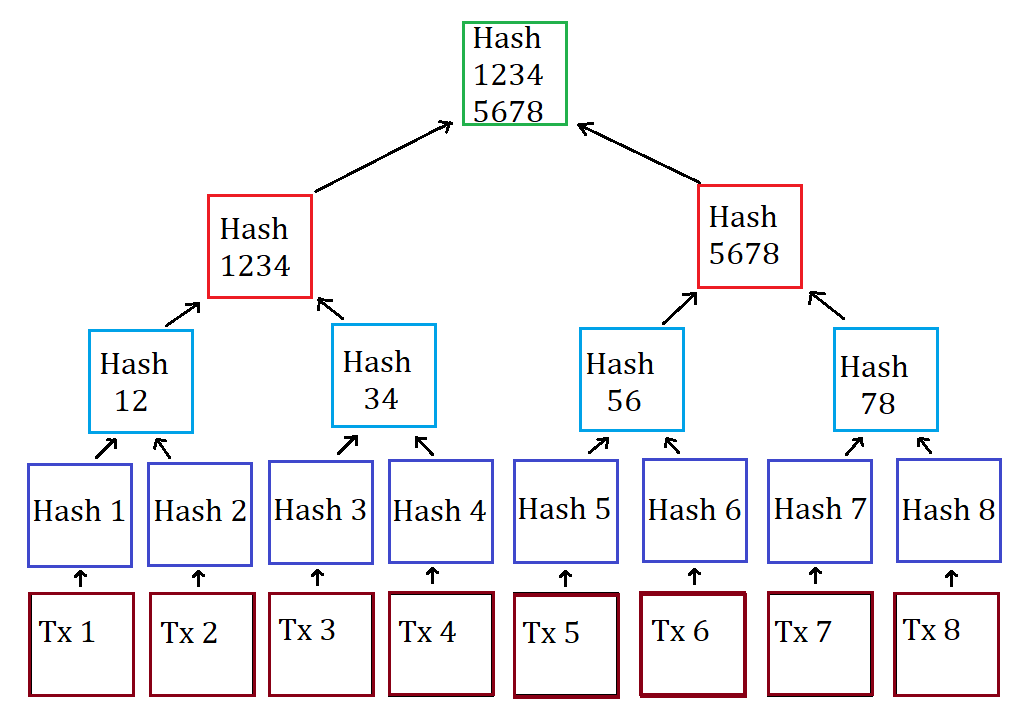
\includegraphics[width=\textwidth]{dependencies/Img/Merkle_Tree.png}
\caption{Merkle Tree example consisting of 8 underlying transactions.}
\label{Merkle_tree}
\end{figure}

A Patricia tree (aka prefix free radix tree) is a different data structure where the \texttt{(key, value)} pairs that are contained within it have the values at the leaf nodes, and the keys let you traverse a path from the root of the tree to the leaves, so that the nodes that share the same prefix in the key also share the same path down the tree from the root to the leaves. See \textbf{Figure \ref{Patricia_tree}} shown below.

\begin{figure}[htbp!]
\centering
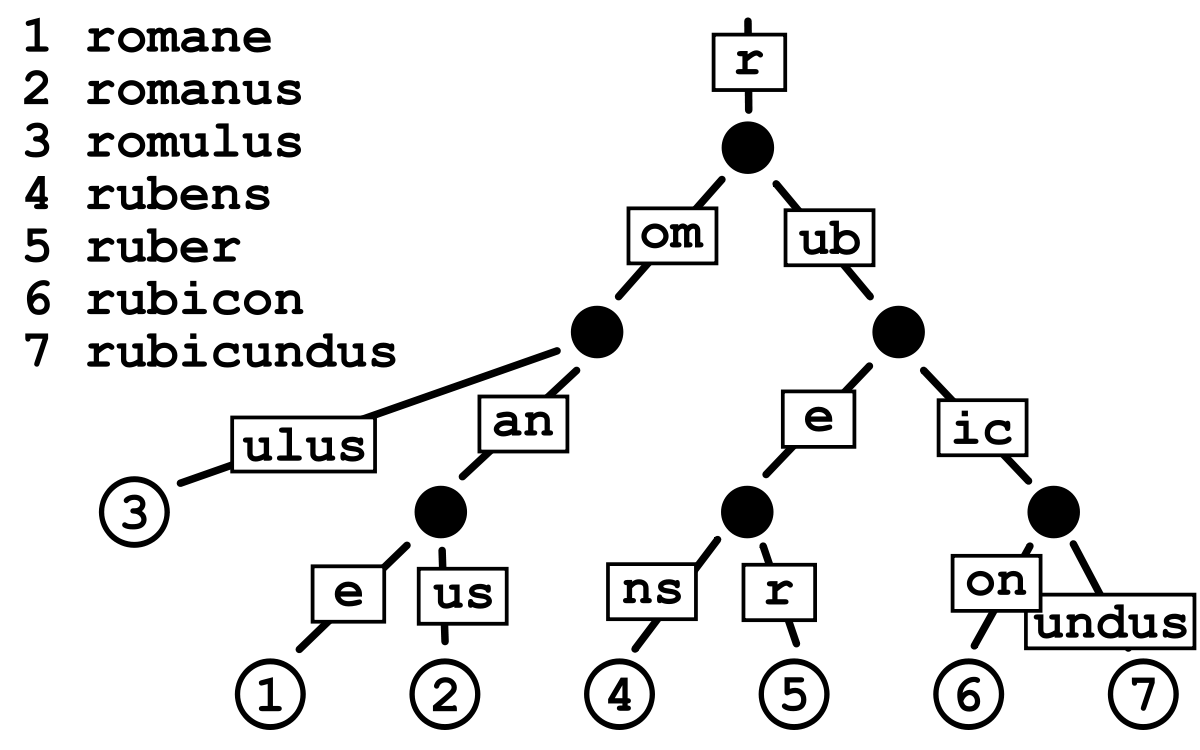
\includegraphics[width=0.76\textwidth]{dependencies/Img/Patricia_Tree.png}
\caption{Patricia Tree example consisting of 7 words.}
\label{Patricia_tree}
\end{figure}

Ethereum uses a combination of a Merkle tree and Patricia tree and it's also modified to specifically suit the Ethereum data structures.
In this particular case, it uses a Hexane-Merkel-Patricia tree which means that each node has 16 children.
There's also a recent proposal to convert this to a binary tree.\\

When looking at the programming languages supported on Ethereum, let's take for example \texttt{Solidity}, there are many common data structures such as arrays, lists, the basic value types, reference types\dots

\subsection*{Consensus Algorithm}

One of the critical core compontents  (perhaps the most critical one) is the consensus algorithm.\\

\textbf{Why is there a need for a consensus algorithm this?}\\

The Ethereum blockchain, as mentioned earlier, consists in many peer-to-peer nodes: these nodes are all talking to each other and trying to agree upon what is the global state of the blockchain.\\

Each of the nodes has a local state, which consits on new blocks being formed containing the transactions that are processed by the node.
But then, everyone on the Ethereum blockchain should agree upon what is the one canonical blockchain that will be used in the future.\\

This is agreement is reached through the \textbf{consensus algorithm}.
Decentralized consensus is critical to any blockchain. In the context of Ethereum it refers to the \textbf{Nakamoto Consensus Protocol} that is adapted from Bitcoin. This protocol addresses the problem of which miners' block should be included next to create the canonical blockchain. There are two components to this: \textbf{Proof of Work} (PoW) and \textbf{The longest chain rule}

PoW is used to determine which entity on the Ethereum blockchain gets to add the next block; \textbf{the consensus algorithm} determines which is the longest chain so far, and all the nodes that are chosen to add the next block to the existing canonical blockchain build upon the existing longest chain.
This is how a blockchain grows in state.\\

The consensus algorithm is used as a form of \textbf{sybil resistance}.
There's this concept of 51\% attack, which consists in the scenario of 51\% of the participating entities colluding.
Then, these malicious entities can change past states (and thus the state transitions) that have been encoded into the blockchain.
This breaks the key property of immutability of a blockchain, thus it is very critical.\\

\subsection*{Ethereum PoW: Present and Future}\label{subsection:EthereumPow}

As mentioned previously, Ethereum Proof of Work is fundamental to how the Ethereum consensus protocol works.
Technically, it is referred to as Ethash, and it's formally defined as

$$(m,n)=\text{PoW}\left(H_\text{\sout{$n$}},H_n,d\right)$$
$$m=H_m\wedge n\leq\frac{2^{256}}{H_d}$$

\qquad where $H_\text{\sout{n}}$ is the new block's header but without the nonce ($n$) and mix-hash ($m$) components; $H_n$ is the nonce of the header; $d$ is a large data set needed to compute the mixHash and $H_d$ is the new block's difficulty value.\\

What a miner has to do is to determine a combination of mix-hash $m$ and nonce $n$ for every block to satisfy the constraint on the difficulty for that particular block.
This is a trial and error process so the miner has to keep repeating the computation until a combination of $m$ and $n$ that satisfies the difficulty is found.
When this is done it means that a sufficient amount of work has been performed by the miner for this particular block, or in other words this indicates that there is proof of work by the miner for this block.\\

PoW is being replaced by what is known as \textbf{proof of stake} (PoS).
With Ethereum it's happening with the transition to Ethereum 2.0 or Serenity (also known as \textbf{the merge}).
The merge is already underway.
This change is important from a security perspective: the consensus algorithm is critical to the economic security of a blockchain, as it is what makes the blockchain resistant to attacks from any of the untrusted parties operating the infrastructure or operating on it.
For now, this security is provided by PoW.

\subsection*{Ethereum Nodes and Clients}

An Ethereum node is a software application that implements the Ethereum protocol specification.
It communicates with other Ethereum nodes on the network in a peer-to-peer fashion.\\

The Ethereum client is a specific implementation of the Ethereum Node.
Withing the Ethereum clients, a specification of the protocol itself (the consensus algorithms, data structures,\dots all these core components) is implemented.

If anyone is running an Ethereum node they're using one of these Ethereum clients that have been built by multiple teams around the world.
The most popular ones are
\begin{itemize}
\item Geth
\item Erigon
\item Nethermind
\item OpenEthereum
\end{itemize}

There have been a lot of transitions and changes.
Some of the clients have been under development, and some of them are way more popular.
Geth is the most popular with more than 80\% of the running nodes.
But, for the sake of the diversity and decentralization of Ethereum, other clients are being supported and being developed as well.
These clients are open source so anyone is free to examine the client code and maybe even contribute to it.\\

Ethereum transactions are sent to the Ethereum Nodes, and these in turn broadcast them across the peer-to-peer network.
This is how Ethereum transactions propagate across the Ethereum network, reach the various nodes, get combined into blocks and result in the blockchain.

\subsection*{Ethereum Miners}

Ethereum miners are entities running Ethereum Nodes on the network.
They are the ones that receive, validate, execute and combine the transactions into blocks.

They also provide a mathematical proof of their computation (proof of work; PoW).
For all this work, if the miner's block gets chosen to be part of the blockchain, then they are rewarded with what is known as a block reward.\\

This block reward is currently 2 ether and it has decreased over time. This is the crypto economics: incentive for miners to participate and to be honest on the Ethereum network.
Along with this reward, they're also rewarded with transaction fees: the ether spent on Gas by all the transactions included in that block.\\

So block reward and transaction fees are the crypto economic incentives that are paid out to the miner whose block gets accepted into the blockchain.

\subsection*{GHOST protocol}

So transactions are sent, and miners validate them.
They combine them into blocks and these blocks are propagated over the peer-to-peer network.
Multiple miners are doing this process simultaneously.
This leads to multiple valid blocks at any level of the blockchain.
The canonical blockchain needs to choose one valid block at any level.
The choice of that valid block is dictated by the ``\textbf\textit{GHOST protocol}'' (the Greedy Heaviest Observed Subtree protocol).
This protocol allows stale blocks up to seven levels in this calculation.
Stale blocks, in Ethereum's nomenclature, are referred to as uncles or armors.

\section{Gas Metering: Solving the Halting Problem}

\subsection*{The Halting Problem}

We talked earlier about Turing completeness and how Ethereum supports a Turing complete programming language.\\

Turing completeness lends itself to a fundamental problem in computer science: the halting problem.
Imagine you have a Turing complete programming language, then the halting problem states that: it cannot be predicted if an arbitrary program in that language with an arbitrary input will ever stop execution for that input.\\

This problem is taken for granted on our personal laptops or on our phones: if there are programs that run into an infinite loop that hangs them, then we just manually kill the execution.\\

In the context of a blockchain however, we are talking about being able to deploy a smart contract that is not going to run on my Ethereum node exclusively, but it's going to run on all the Ethereum nodes in the blockchain.
With that in mind, if any of those smart contracts ran into an infinite loop, then the whole infrastructure would come to a grinding heart, which is obviously undesirable.
We would not make further progress and everything would come to a standstill.\\

The way in which Ethereum deals with this issue is constraining the resources that are given to the smart contract on the Ethereum node by metering them through the concept of Gas.

\subsection*{Gas Metering}

The EVM runs smart contracts, which have machine code instructions.
Every single one of these instructions has a predetermined execution cost in Gas units.
So when a transaction triggers the execution of that smart contract, and the smart contracts starts executing those instructions, then the Gas units for those instructions are ``consumed'' by the smart contract.
This is the concept of Gas metering within a smart contract, where it accounts for every instruction (it could be a computational instruction, a data access,\dots\, All those instructions consume Gas units from the transaction).\\

This implies that a transaction that triggers a smart contract has to include a specific amount of Gas as required by the logic of the smart contract.
Depending on what logic needs to be executed by said smart contract, there is a limit to the gas: a certain amount of Gas units are required for a particular flow, so if a transaction is triggering that it must include so many Gas units.
In fact, even if the transaction is just triggering a transfer of value, it has to supply the amount of Gas required for what it is triggering.\\

If the Gas that is required during the execution of the smart contract exceeds what is supplied, or if it exceeds the limit, then the EVM will terminate execution and the transaction will fail.
This is fundamental to how Ethereum works, since there is a need to bound the use of resources by anyone interacting with a smart contract that runs on all the blockchain nodes all over the world.\\

Up until this point, all we have talked about is the units of Gas that have to be provided.
However, Gas itself has a price, which is measured in Ether.
So this Gas price is not fixed as it depends on the supply and demand of Ether.
In this context it depends on the demand for the block space within Ethereum, and if there are many applications (many smart contracts) and/or users competing for that block space, then the Gas price can increase vastly.
So just like the automobile analogy (which requires Gas or petrol, and with a fixed amount of petrol one can drive a certain amount of kilometers), the petrol is the equivalent of the Gas units in Ethereum (which allows to run a transaction in a certain number of instructions within the smart contract based on the amount of Gas you supplied).
But the Gas price, similar to the price that you pay in Gas stations (petrol bunks) is different and depends on the supply and demand.\\

This Gas mechanism has recently been updated; take a look at EIP1559 (Ethereum Improvement Proposal 1559).\\

The take home message for this section is: one needs to obtain gas, which is obtained by purchasing Ether.
A transaction requires gas, and if it exceeds the amount of Gas that is supplied, then the transaction fails.
But if there is more Gas than what is required, that is supplied as part of the transaction, then the remaining Gas is sent back to the sender who executed the transaction as part of the protocol. 

\section{Web 2.0 Vs. Web 3.0: The Paradigm Shift}

In this section, we are going to assume that you are familiar to some extent with Web2 and most of the content will be focused on Web3 and the differences with Web2.

\subsection*{Objectives of Web3}

The idea of Web3 is for it to be a permissionless, trust minimized and censorship resistant network for transfer of not only information but also value.\\

Privacy and anonymity are again very big motivating factors in Web3 and have a huge implication on how we think about security in this space and how we can actually conceive implementing various security measures.
However it isn't a completely fresh start: there are a lot of Web2 security principles, best practices and software engineering best practices that have been researched, experimented, developed and refined over the last 3 or 4 decades that still apply very much to Web3.\\

In the Web3 world the aspirational goal is that of borderless, permissionless innovation and censorship resistance. This inspires all the applications, smart contracts or any other off-chain components to be open and composable by design

Another 
Composability means designing components and applications in a modular way, so that other modules (or other applications) can interface with them to increase the utility that is got from either of the two components. This has to be done in a way that is very easy, permissionless and effortless. Again, going back to the Web2 space, a lot of the work that has happened, a lot of the applications that are built by the various enterprises, for various reasons such as protecting their business interests, are designed in such a way that they work well within their ecosystem or their suite of products, and they're not really meant to be very composable or very interactive with other applications or other components from other entities or other vendors (potentially their competitors).\\

In the Web3 world the aspirational goal is that of borderless, permissionless innovation and censorship resistance. This inspires all the applications, smart contracts or any other off-chain components to be open and composable by design. This means that anybody (any user, any part of the world) can deploy applications and interact with it (be it contracts, be it any other component). This drives innovation in the Web3 space, which is great and has resulted in a very accelerated innovation and compressed time. Again this has implications to to how security is thought of and what is practically possible with security in this space. When you have this unconstrained composability, where any smart contract, any application that is deployed can be acted upon and be combined or connected with any other smart contract on the chain, then it leads to sort of an explosion of the dependencies and configurations that are possible. This makes characterizing Web3 vulnerabilities and exploit scenarios very challenging, because it requires really a very deep knowledge of all these interacting composable components along with their very different constraints that could change because of composability itself, and their configurations could be affected by interactions with other components.

Having said that, there are still many aspects of Web3 security which are really a paradigm shift.

\subsection*{Open-source \& Transparency}

Due to Web3's ethos (or the design approach) towards everything here being open source and transparent, the way it is thought about the security of the ecosystem has to be changed.\\

We have known open source in the Web2 world for several decades, so that's not very new.
But from a approach perspective, in the Web2 space we do see most of the products, or many of the products, being proprietary from a licensing and from a source code availability perspective.
The Web3 ethos stems from the permissionless aspect, the trust minimization aspect and the censorship resistance aspect.\\

In the context of smart contracts, they're again expected to be open sourced and also expected to be verified contracts. In this case it means that the bytecode (machine instructions) of the contracts deployed on the blockchain are expected to be source code verified using one of the services available (such as \href{https://etherscan.io/}{Etherscan}).
This means that the source code of the contract is the same one that was compiled, deployed and that users interact with.
That verification is something critical and expected by default in this space.\\

Remember that everything that happens in the blockchain is transparent; anyone can actually run an Ethereum node so that you don't even have to rely on a block explorer or any service like that (more on that in upcoming secitons).
You can look at transactions as they happen in real time on the blockchain, you can also look at transactions that are waiting to get into the blockchain (through mempool explorers).
One can even do that by running an Ethereum node themselves. 
\textbf{There is no security by obscurity}.

\subsection*{Code Immutability}

In the context of a blockchain being immutable (because of all the blocks being linked with hashes), PoW and what it requires for somebody to go back in time and change one of the blocks or any of its contents, which contributes to the economic security and the immutability aspect of the blockchain.\\

When it comes to code, the contracts that are deployed on the Ethereum blockchain are designed in a way to be immutable as well.
This means that once a contract code is deployed, it is technically considered immutable: it cannot be changed (at least in theory).
There are some exceptions, so theoretically it can done, but from a design perspective (from an ethos perspective) this is not desirable.
This code immutability affects the way in which security is handled.\\

As it is already widely known, software will have bugs: one cannot prove the absence of bugs, or the absence of vulnerabilities or errors in a piece of software.
Immutability affects this to a great extent: we know that bugs will exist and, if you cannot change the contracts, then how do we fix the code and redeploy the fixed code as we've been used to in the Web2 world (where we keep getting updates to the operating system or to the different apps continuously to fix bugs, optimizations and so on)?\\

This is something very fundamental to Ethereum or the Web3 space that we have to keep in mind.\\

There are practical exceptions: the deployed contract can be modified: the functionality can be modified.
This can be done in three ways.

\begin{enumerate}

    \item The contract can be modified and redeployed at a new address, but then you would have to carry over all the state.
    And all the users interacting would have to migrate to interacting with the new address.\\

    This is typically considered impractical but it can theoretically be done.

    \item The modified contract (after bugfix or a version 2) can also be redeployed as a new implementation of what is known as a proxy pattern: the proxy contract points to an implementation contract, and that implementation can be modified.\\
    
    This is the most commonly used approach to contract upgrading, and again this has huge security applications if it is not done right, if it is not done in a trustworthy manner or if there are certain best practices that are not followed.

    \item By using the \texttt{CREATE2} opcode, it allows updating a contract in place at the same address using the same unit code that was used to initialize the contract.

\end{enumerate}

We are going to further elaborate on the concepts briefly mentioned here on upcoming sections.

\subsection*{Client-Server Vs. Peer-to-Peer}

The pivotal difference between Web2 and Web3 is their underlying paradigm.\\

\textbf{Web2} relies on the \textbf{client-server paradigm}: we are used to employ cloud services that have servers running, which we interact with using our clients (laptops, phones, smart watches\dots) that are \textbf{centrally managed}, i.e. you have all these corporate entities that determine what the infrastructure is, what the products are and what the next versions of the products will be.\\

Applications are centrally rolled out and the consumers use them, but they do not have a say in how the infrastructure is managed or how the applications evolve.
Sometimes, users don't even have a say as to what kinds of applications can be deployed on the infrastructure: there is a latent \textbf{censorship on Web2}.\\

The former scenario is something that Web3 is trying to get away from: it's trying to go back to the original vision of the web which was for it to be completely peer-to-peer without centralized entities that can dictate what can be done on the platform, what can be deployed or who can use it.\\

The idea is employing peer-to-peer communication not only for computing power but also for storage and network, which are the building blocks of Web3.
In the case of Ethereum, the peer-to-peer infrastructure that supports these components is known as the \textbf{Ethereum triad}

\begin{itemize}
    
    \item\textbf{Comouting power}: Ethereum itself; Ethereum as a blockchain is used for decentralized compute.
    
    \item\textbf{Storage}: Swarm.
    
    \item\textbf{Network}: Whisper (now known as Waku). 

\end{itemize}

\subsection*{Business models}

Web2 business models are built around \textbf{freemium models} where the basic application is free but if you want to upgrade, you have to pay up.
A lot of the business models (Google, Facebook especially) are built around advertising, where the product is free.
In some sense, the user becomes the product and the interactions (the data that the user shares with those platforms) is monetized in the form of advertisements that are being delivered to the user.
This is something that we've just got used to and we don't even pay attention to anymore.\\

In Web3, since everything is decentralized, there has to be some incentive for users to deploy the nodes and to contribute to the development of the code, clients, smart contracts and applications.
This is driven by what is known as ``\textit{incentivized participation}'', which goes back to the concept of crypto economics.
This has big implications to how security works because there is no real centralized entity that can deal, manage and do instant response.

\subsection*{Programming languages}
Programming languages are critical because they are the means of how projects implement their ideas, deploy them and let users interface with them.\\

Again, programming languages are fundamental to the security of any product, any architecture if you will.
In the case of Web2 there have been numerous programming languages, being some of them way more popular than the rest: it started with \texttt{C} and \texttt{C++} during the Unix days 30 or 40 years ago, and since then we have seen different declarative languages, subject-oriented languages and scripting languages.
Some of the most popular ones have been \texttt{Javascript} and more recently \texttt{Go}, \texttt{Rust} and even some unique languages such as \texttt{Nim}, that have been used to implement Ethereum 2.0 clients recently.\\

All those languages are still applicable to the Web3 space, Because Web3 is a combination of smart contracts that run on the blockchain and web interface component (which is how users interact with the contracts on the blockchain).
When it comes to the web component, all the Web2 languages are relevant.
A lot of them are popular even here in terms of the interface, but also in terms of the tooling that is used for the development of smart contracts themselves.\\

Smart contracts themselves have a special language.
In the case of Ethereum, that's \texttt{Solidity}: it is the most widely used language for writing smart contracts on Ethereum.
There are others, like \texttt{Vyper}, that are gaining traction, but for the majority of the smart contracts that we see deployed, \texttt{Solidity} is that language.\\

The smart contract languages were created specifically for Web3, and specifically for Ethereum in this case. So the security features of those languages have obviously huge implications to the security of the smart contracts themselves and the applications that are built on top of them.

\subsection*{Applications in Web3: \DJ Apps}

Building applications on a decentralized infrastructure (i.e. a blockchain) will cause such applications to be fundamentally different from the mobile applications or the desktop applications that we are used to today (as we can already guess by looking at the programming languages and code immutability in Web3).
These applications are referred to popularly as decentralized application or \DJ App.\\

These applications rely on a concept that is very unique to Web3: \textbf{on-chain} and \textbf{off-chain}.

\begin{itemize}
    
    \item\textbf{On-chain} means something that is running or executing on the blockchain or within the blockchain's execution environment.
    
    \item\textbf{Off-chain} is something that is running outside the blockchain.

\end{itemize}

In the Web2 space everything is off-chain because, obviously, there is no concept of blockchain.
However, in order to function, the Web3 space makes use of an off-chain component combined with an on-chain component.\\

The off-chain component is all the Web2 or ``\textit{the glue}'' that binds the web interface to the smart contracts that are running on-chain.
This distinction is critical when thinking about security.\\

To put it simple, a \DJ App combines a web app/web front-end or a mobile app (the off-chain component) that interacts with a smart contract on the blockchain (the peer-to-peer infrastructure which is a combination of compute, storage and network; the on-chain component).
In many cases we have one or more of any of the mentioned.\\

In the case of Ethereum, what is peer-to-peer is the compute part and the peer-to-peer storage aspects (such as IPFs and some of the other protocols that we won't talk about).\\

The security of Web3 has to think about the security implications of anything running or interacting off-chain with that running on-chain as well.
It's not just smart contract security but also the security of the off-chain web or mobile app components that interface with the on-chain components (the smart contracts).\\

The main difference however between Web2 and Web3 security is the on-chain component of course.
We will need to think about at the pitfalls that are unique to smart contracts and look at the best practices.

\subsection*{Unstoppability \& Immutability}

Another difference between Web2 and Web3 is that the Web3 applications and infrastructure are unstoppable and immutable.\\

We talked about \DJ Apps and how they run on a decentralized infrastructure.
The goal is even for the governance of these protocols and infrastructure to be decentralized, this means that there is no single entity that can unilaterally decide to make changes, to start something, to stop the application (be it adapt be the protocol, be the surrounding infrastructure or the governance itself).
Specifically, in the case of smart contracts, there shouldn't be a single entity.\\

This could be the the project team itself that has built out this application or the contracts: they shouldn't be unilaterally allowed to change, stop and withdraw funds. 
This stems from the trust minimization motivation and the censorship resistance aspect.\\

They are all very interconnected aspects and as you can imagine they have huge implications to when it comes to upgrading the contracts, fixing the bugs or doing anything with the smart contracts once they're deployed; because they are expected in theory, by motivation and by design (codewise; remember the code immutability we talked about earlier) to be unstoppable and immutable.\\

From a security perspective, this makes it hard to deploy the software because once you do it, if there are any vulnerabilities found, it's very hard to do an instant response (just what we talked about on code immutability).
The latter is something we take for granted in the Web2 world, where we get software updates even without our knowledge.\\

In the case of Web3, and particularly Ethereum smart contracts, this has huge implications to how we think about design and operationalize security.
This is the ultimate goal, in practice, as we go through different stages of progressive decentralization.
These things are evolving, so the best practice right now is to do something known as a ``\textit{guarded launch}'' (basically initially limiting the functionality of the \DJ App for monitorization purposes).
For now the best practice is to have the ability to make changes, to upgrade the contracts, to have an emergency withdrawal function, to remove the tokens in case there is an emergency.
It's sort of the stop cap measure as we progress towards complete decentralization.
Once we have enough confidence that the contracts are running and there are no bugs, vulnerabilities or exploits, then a lot of these things are disabled in the code: the kill switches or the credibility aspects the governance\dots\\

All these things are in a progressive manner made more decentralized over time.

\section{Decentralization}

\textbf{What does decentralization really mean?}\\

This term is used very casually although it has huge implications to how we think about security, even for smart contracts.
There is a definition put forth by Vitalik in his article on decentralization.
There are three types of decentralization

\begin{itemize}

    \item\textbf{Architectural decentralization}: it refers to the hardware (the physical computers); who runs them, owns them, who is managing them, who can start them and stop them.
    This can be done in a decentralized fashion or not.

    \item\textbf{Political decentralization}: it refers to the people behind the hardware or what is commonly referred to as ``\textit{wet ware}''.
    Who are the individuals or the organizations who control the hardware or the infrastructure?
    Is it just one individual or is it a group of individuals?
    Are the colluding or are they independent and decentralized?

    \item\textbf{Logical decentralization}: it refers to the software: used to build out the applications (the framework itself, the Ethereum code, the protocol itself, the data structures in it, the smart contracts or any other software that runs in that stack).
    Is that decentralized?
    Is it a monolithic entity that cannot be split apart and used in a decentralized fashion?

\end{itemize}

All of these have security implications.

\section{Cryptography, Digital Signature and Keys}

Most of you know tat there are two classes of cryptography: \textbf{symmetric cryptography} (there is a single key shared between aprties) and \textbf{asymmetric cryptography} (there is a key pair: public key and private key). In the case of Ethereum, the cryptography that is used is all about digital signatures and not as much about encryption at a protocol level.
These digital signatures however depend on the concept of public key and private key.

\subsection*{Private Key}

The private key is a secret and the owner has to keep it in a safe place.
In the case of Ethereum, it's a 256 bit private key.
It's effectively a random number and it's used to derive the public key.

\subsection*{Public Key}

The public key, however, is not secret.
It is a point on the elliptic curve calculated from the private key using elliptic curve multiplication.
The public key is used then to derive the address of an Ethereum account (by hashing the public key by means of the keccak-256 cryptographic hash function and taking the last 20 bytes of the output; it is a very simple calculation) and it is also used by others to engage in cryptographic protocols with the owner of the private key.\\

It is important to remember that the public key cannot be used to derive the private key.
This is should be something obvious to security, because otherwise if the public key could be used to derive the private key, then this key pair system would not deliver any kind of security.\\

This is the high-level aspect that you need to remember: there's a private key, which is used to obtain the public key, and from the public key we derive the address of the Ethereum account.

\subsection*{keccak-256}

We mentioned earlier that the keccak-256 cryptographic hash function is used in the steps of computing the EOA address from the public key.\\

keccak-256 is actually the cryptographic hash function that is used by Ethereum.
It is very closely related to the SHA3 (the secure hash function).
The latter was finalized as the standard by MIST (National Institute of Standards and Technology) and in the case of Keccak-256, it was the winning candidate for the SHA3. However, the SHA3 standard was adopted instead.\\

keccak-256 is critical to a lot of the functioning of the Ethereum protocol and smart contracts as it's a fundamental primitive to how computation in many ways is done on Ethereum.

\subsection*{Digital Signature: ECDSA}

The digital signature algorithm used by Ethereum is the same one that is used by Bitcoin.
It is known as ECDSA: \textbf{Elliptic Curve Digital Signature Algorithm}.
Elliptic Curve Cryptography is an approach to public key cryptography based on a particular algebraic structure of elliptic curves over finite fields.\\ %% ELLIPSIS expand on this?
In the case of Ethereum, the particular elliptic curve used is known as Secp-256k1 (this refers to the parameters that are used for the elliptic curve).\\

Digital signatures are  fundamental to how Ethereum works, are powered by public key cryptography (asymmetric cryptography) and habe three main purposes:

\begin{enumerate}

    \item\textbf{Authorization}: inclusion of the signature proves that the owner of the private key who created the signature (and who by implication is the owner of the sending Ethereum account) has authorized the transaction to spend the ether or to execute the contract that it is targeted.

    \item\textbf{Non-repudiation}: once the signature has been included, it cannot be later denied that authorization was granted for that transaction to execute.

    \item\textbf{Integrity}: it proves that the transaction data has not been modified or cannot be modified by anyone after the transaction has been signed.
    This is one of the fundamental security properties.

\end{enumerate}

\section{Ethereum State \& Account Types}

Ethereum state is a mapping from the address of the Ethereum accounts to the state contained within it as a data structure.
It is implemented as a \textbf{Modified Merkle-Patricia Tree}: a combination of a Merkle tree and a Patricia tree with some changes that are specific to Ethereum.\\

Each of the Ethereum accounts has a unique 20 byte address associated with it, which is used by accounts to ``talk to each other''.
Addresses are critical to how messaging works within the Ethereum protocol and how the accounts engage in transfer of value or information, since accounts need to be able to refer to each other using their addresses.\\

In addition, accounts have four fields:

\begin{itemize}

    \item\textbf{Nonce}: a counter that's used to make sure that each transaction can only be processed once used to prevent replay attacks.
    
    \item\textbf{Balance}: a number representing the amount of Ether that the account has at any point in time.
    
    \item\textbf{Contract code}: smart contract code (absent in Externally Owned Accounts).
    
    \item\textbf{Contract storage}: associated smart contract storage (absent in Externally Owned Accounts).

\end{itemize}

\subsection*{Account types}

Ethereum has two account types:

\begin{itemize}
    
    \item\textbf{Externally Owned Account (EOA)}: it is an account that is controlled by a private key.
    Anyone who has a private key can create a digital signature that can be used to control the Ether that is present in an EOA.
    These signatures can be used to sign transactions from the EOA, which in turn can trigger messages from the EOA to other accounts.
    These messages can result in a transfer of value or they can trigger smart contracts.\\

    An EOA does not have any associated code or storage.

    \item\textbf{Contract account}: it is an account that is controlled by the code that is contained within that account.
    
    Unlike EOAs, contract accounts have an associated smart contract code and storage.
    Whenever the contract account receives a message, it triggers the code present and accesses any internal storage associated with it.
    When the code runs it can send messages to other accounts or even create new contracts.

\end{itemize}

In this sense, smart contracts can be thought of autonomous agents as they're always present in the execution environment of the Ethereum blockchain.
They're always ready to be triggered by a transaction or a message that is sent to them.
Through their contract account they have access to the Ether balance and the contract storage.
The execution of the code results in manipulation of this balance and the contract storage.

\section{Transactions: Properties and Components}

Transactions are \textbf{signed messages} that originate outside of the Ethereum blockchain.
They are \textbf{triggered by EOA}s (that are managed or controlled by a private key).
The trigger happens to be the digital signature, derived from the private key.
These transactions are transmitted by the Ethereum network and they trigger state changes on the blockchain.
In fact, Ethereum is fundamentally a transaction based state machine, as only transactions are capable of triggering state changes.

\subsection*{Properties}

\begin{enumerate}

    \item Transactions are \textbf{atomic}: they run from the beginning to the end completely, it's either all or nothing.\\

    So the side effects of the transactions are only reflected in the blockchain if they run to completion.
    If they don't, nothing that they do is reflected on the blockchain and it's as if the transaction never happened.
    In other words: transactions cannot be divided or interrupted with some of the partial state being reflected on the blockchain and the rest of it not.\\

    This contrasts withtraditional computing environments where a particular process or a particular control might be interrupted, gets context washed out and then something else (a different process or a thread) executes and then the original context is brought back.
    None of that happens within the context of Ethereum.\\

    \item Transactions are \textbf{serial}: they're executed one after the other, sequentially without any overlapping.
    There is no parallelism when it comes to the execution of transactions.

    \item Transaction \textbf{inclusion}.
    When a user submits a transaction, what is the warranty that it gets included within one of the blocks on the Ethereum blockchain?
    This property is controlled by entities on the Ethereum blockchain known as miners.
    They run Ethereum nodes and decide which transactions are included within a block.
    This depends on multiple factors, the key ones being the congestion on the Ethereum network (or in other words, the other transactions that are competing for the same block space) and the Gas price that the user decides to use for the particular transaction.

    \item\textbf{Inclusion order}.
    It refers to the specific order of the transactions included within a block.
    Again, th is chosen by the miners and, similarly to inclusion, is determined by factors of congestion and Gas price.\\

    The key takeaway of properties 3 and 4 is that there are entities known as miners on the blockchain who get to decide which transactions get included within a certain block and the specific order of the transactions within that block.    

\end{enumerate}


\subsection*{Components}

Transactions contain seven components:

\begin{enumerate}

    \item\textbf{Nonce}: the name is an abbreviation for ``a number used only once''.
    It's a sequence number that, as part of the protocol, is incremented in a particular fashion (it changes for every transaction).
    The application of the nonce is prevention of replay attacks (i.e. replaying the same transaction over and over again).\\

    In the case of an EOA, the nonce value is equal to the number of transactions sent from that account.
    In the case of a contract, it is equal to the number of other contracts created by this contract account.
    
    \item\textbf{gasPrice}: the price for every Gas unit that the sender is willing to pay for a particular transaction.
    It's measured in $\text{wei}/\text{gas}$.\\
    
    The gasPrice is not fixed by the Ethereum protocol.
    The higher the Gas price that the the sender is willing to pay for this transaction, the faster the particular transaction gets included by the miner into a block in the blockchain.
    This price depends on the demand for the block space at the point in time when the transaction is submitted.\\

    The reason for this is that there is a limited amount of space in the block, so there's only a limited number of transactions (as determined by the Gas used by each one of them) that can be included within this block.

    \item\textbf{gasLimit}: the maximum number of Gas units that the sender is willing to pay for a particular transaction.
    
    This depends on the type of transaction that is being sent.
    If it is a simple Ether transfer then it costs 21000 Gas units.
    But if it is a transaction that is targeting a particular contract (or a particular function of the contract) then the required amount of gas is higher.\\

    If sufficient Gas (in the form of Gas limit) is not set for the transaction (if it's less than what is required to), then it results in what is known as an \textbf{out of Gas exception} (OOG Error) and that transaction fails.
    The way it works is that for any transaction that is being sent by a sender, there is an estimated Gas that needs to be sent as part of the transaction.
    If that estimated amount of Gas is not sent then it leads to the exception.
    If there is excess gas, then the remaining Gas is sent back to the sender.

    \item\textbf{Recipient}: the destination 20 byte Ethereum address for a transaction (i.e. the destination account that this transaction is targeting).\\
    
    This could be an EOA address or a contract address, it depends on the target of that particular transaction.
    It could be any address on the Ethereum blockchain, and the protocol itself does not validate these recipient addresses in the transactions.\\

    So one can send a transaction to any address and that address might not even have a corresponding private key, nor the contract that the sender expects to have.
    Thus, all such validation should be done at the user interface level.
    That validation is critical for security reasons (more on that in later chapters). Note that this recipient is really the target address.\\

    There is no ``from address'' that is a component of the transaction.
    The reason for this is that the ``from address'' can be derived from the ECDSA signature components $v$, $r$ and $s$: they can be used to derive the public key, which in turn can be used to derive said address.

    \item\textbf{Value}: the amount of Ether (in wei) that the sender is sending to the recipient address.\\

    What happens with such funds depends on the recipient: if it happens to be in EOA, then the balance of that account will be increased by this value and the sender's balance correspondingly decreases.
    If it hapens to be a contract account, then what happens depends on any other data present as part of this transaction (i.e. the contract function being invoken with the transaction data).\\
    
    If there is no data being sent as part of this transaction, and the destination happens to be a contract account, then the contracts' \texttt{receive} or \texttt{fallback} function (if they were defined or if they are present; more on that in the upcoming chapters) are triggered and thus, what happens with the received Ether depends on their implementation.\\
    
    If there is no \texttt{fallback} function, then the transaction results in an exception and the Ether, that is sent as part of the transaction, remains with the sender account.

    \item\textbf{Data}: payload of variable length and binary encoded (as per the format required by Ethereum) that is sent as part of this transaction.\\
    
    This field is relevant when the recipient is a contract account. As mentioned previously, the data in that case contains the contract function that is being targeted by the transaction plus the specific arguments that are relevant for said function.

    \item\textbf{$\boldsymbol{v}$, $\boldsymbol{r}$ \& $\boldsymbol{s}$}. The ECDSA signature is 65 bytes in length and has three subcomponents: $v$, $r$ and $s$.
    
    \begin{itemize}
        
        \item $r$ and $s$ represent the signature components.
        They are 32 bytes in length each (adding up to 64 bytes).

        \item The final subcomponent, $v$, is the recovery identifier.
        It's just one byte and its value can be either 27 or 28, or it can be twice the value of chain ID ($2\times\text{ID}_\text{chain}$) plus either 35 or 36.\\

        The chain ID is the identifier of the blockchain.
        In the case of the Ethereum mainnet chain, $\text{ID}=1$.

    \end{itemize}
    
\end{enumerate}

For a particular transaction, the Ether used to purchase Gas is credited to the beneficiary address that was specified in the block header (more details on this are found in the upcoming sections).
Then there's also a concept of a Gas refund: the difference between the Gas limit and the Gas Used is refunded back to the sender of the transaction.
This is done at the same Gas price as indicated in that transaction.

\section{Contract Creation}

We mentioned that a transaction can result in contract creation.\\

The creation transaction is a special one because it's sent to a special destination address called ``\textit{the zero address}''(\texttt{0x0} address), which is an address that has zero in all its bits.
This zero address is treated in a special maner within Ethereum, and it becomes critical to some of the smart contract security properties.\\

It contains a data payload which represents the byte code of the contract that is being created, and it may also contain an optional Ether amount in the value field, in which case the new contract that is being created, will have a starting balance equal to this Ether value.

\section{Transactions, Messages and Blockchain}

\subsection*{Distinction between Transactions and Messages}

So far, we have used both the terms Transaction and Message interchangeably, but in the context of the protocol they are actually very different:

\begin{itemize}
    
    \item\textbf{Transactions}: originate off chain (by an EOA when an external actor, that is, external to the blockchain, sends a signed data package onto the blockchain) and target an entity on the blockchain.\\
    
    This transaction can trigger a message that can do one of two things:

    \begin{enumerate}

        \item It can trigger a message to another EOA, in which case it leads to a transfer of value (transfer of Ether).

        \item It can trigger a message to a contract account, in which case it leads to the recipient contract account running its contract code and doing whatever the code is intended to do.

    \end{enumerate}    
    
    \item\textbf{Messages}: the origination and the destination are both onchain.
    Messages can be triggered in two ways:

    \begin{enumerate}

        \item externally by a transaction.
        The destination of that message could be another EOA or another contract account.

        \item internally within the EVM.
        This happens when a smart contract executes the call family of opcodes and that leads to the recipient contract account running its code, or value transfer to the recipient.

    \end{enumerate}

\end{itemize}

\subsection*{How to build a Blockchain}

Blocks are batches of transactions that are grouped together plus the hash of the previous block (a cryptographic hash that is derived from the previous flux data), creating thus a ``chain'' among the blocks.
This is how at high level a blockchain is constructed, and it is also the fundamental reason why a blockchain is considered immutable, which lends itself to the blockchain's integrity.\\

The reason for that is because if someone were to change any component of a historical block (any of the transaction data: the destination or any other aspect) then that change would affect all of the following blocks: all the hashes that are included in the following blocks would be different from the hash of the modified block, and this is something that anybody running the blockchain or looking at the blockchain would notice.
That would break the the immutability of the blockchain.\\

To preserve the transaction history, blocks are ordered. Therefore, every new block created contains a reference to its parent block and similarly, transactions within the blocks are also strictly ordered.
All these critical aspects are the reason why the integrity of a blockchain is maintained and prevents any fraud from happening.

\subsection*{Block Header}

So far we have said that the blocks in the Ethereum blockchain contain transactions, but there's more to it: every block contains a block header along with the transactions.
The headers of the Ommer's blocks.
Each block header itself has several components to it that are critical to how the Ethereum blockchain functions.
They contain several things such as:

\begin{itemize}

    \item\textbf{The parent hash}: the hash of the parent block's header.
    This is what chains the blocks and the Ethereum blockchain together to make it immutable and provides the fantastic integrity property of the blockchain.

    \item\textbf{The Ommer's hash} %%ELLIPSIS elaborate on this?

    \item\textbf{Beneficiary address}: the address of the Ethereum account to which the block reward for mining this block and all the transaction fees collected from the mining of the transactions included in this block are transferred to.
    This address is typically controlled by the miner who has mined this block.

    \item\textbf{stateRoot}: one of the three root hashes of the modified Merkle-Patricia tree.
    These root hashes are 256 bit in length.\\
    
    The manner in which the state root is derived is critical to how the Ethereum state is captured within the blockchain: the leaves of the state root are \texttt{(key, value)} pairs of all the Ethereum address accounts.
    The keys are the Ethereum addresses of the accounts and the values represent the Ethereum state within that account.\\
    
    Recall that every Ethereum account has four fields: a nonce, a balance, a codeHash and a storageRoot.
    If that account happens to be an EOA, then the codeHash and storageRoot don't really matter (they don't contain anything in them).
    But if that account happens to be a contact account, then the codeHash has the Keccak-256 hash of the code that is contained within that contract account, and the storageRoot of that contract account has the rootHash of another Merkle-Patricia tree where the leaves represent the storage that is associated with that contract.

    \item\textbf{transactionsRoot}: one of the three root hashes of the modified Merkle-Patricia tree, where the leaves represent the transactions.
    Also 256 bit in length.

    \item\textbf{receiptsRoot}: one of the three root hashes of the modified Merkle-Patricia tree, where the leaves represent the transaction receipts.
    Also 256 bit in length.\\

    \textbf{But what is a transaction receipt?}\\

    A transaction receipt can be thought of as the side effects of a particular transaction that are captured on the blockchain.
    Besides any changes to the account state that transactions might make, there are other side effects that are captured on the blockchain for this particular transaction.
    It is a tuple that contains four items:

        \begin{enumerate}

            \item\textbf{The cumulative Gas used}: the total Gas used in the block up until right after this particular transaction has happened, so in some sense it captures the ordering of the transactions within the block.

            \item A \textbf{set of logs}: related to the concept of events in \texttt{Solidity} (which we will study in the \texttt{Solidity} chapter). 
            These are events that can be generated by any transaction that is captured on the blockchain. 
            They're really critical to how off-chain components, user interfaces and other components monitor what's happening with a smart contract.

            \item The \textbf{Bloom filters} specifically associated with those logs: they capture the indexed parameters for every event, so that one can query particular parameters of that event in a faster manner.

            \item A \textbf\textit{status quo}: what really happened with the transaction.

        \end{enumerate}

    \item\textbf{LogsBloom} %%ELLIPSIS elaborate on this?

    \item\textbf{dificulty}: difficulty of the block in the context of PoW.

    \item\textbf{block number}: the number of blocks that have been mined so far right.
    This number sort of indicated the position of the block within the blockchain.

    \item\textbf{gasLimit} (called Block Gas Limit under more formal contexts): the Gas limit that's specific to this block.
    This concept is essential to Ethereum as it dictates \textbf{the number of transactions that are added in this block}\\

    This concept is different from the Gas limit which we talked about earlier that was specific to the transaction.
    This Block Gas Limit refers to the total Gas that is spent by all the transactions in that block and this effectively caps the number of transactions that can be included within that block.\\

    So the block size is in fact not fixed in terms of the number of transactions, but it's fixed in terms of the Gas used by all the transactions.
    The reason for that is thst every transaction can consume a different amount of Gas.\\

    The Block Gas Limit is set by the Ethereum miners in a very interesting way: by voting on the blockchain.
    This is currently set to 15 million and it has also changed over time, depending on the miners' voting.
    It also represents the level of demand there is for the block space on Ethereum.

    \item\textbf{gasUsed}: the total Gas used by all the transactions in this block.

    \item\textbf{extraData} %%ELLIPSIS elaborate on this?

    \item\textbf{timestamp}: (derived from the unix time) indicates at what point in time was the block was mined.

    \item\textbf{mix-hash}: critical component of the PoW.
    See \textbf{subsection \ref{EthereumPow}}.

    \item\textbf{nonce}: critical component of the PoW.
    See \textbf{subsection \ref{EthereumPow}}.
\end{itemize}

\section{EVM (Ethereum Virtual Machine) in Depth}

The EVM is the execution component of the Ethereum blockchain: is the runtime environment where all the smart contracts run.
Recall that EVM is a quasi turing complete machine: it's turing complete because the underlying programming language supports arbitrary logic unbounded complexity, but it's also bounded by the amount of Gas provided as part of every transaction.\\

The Ethereum code runs within the EVM and it is written in a low level stack based language referred to as the EVM Machine Code.
This code consists of a series of bytes (therefore referred to as a bytecode) where every byte represents a single operation.
So the opcodes are very simple and each of them is a single byte.

\subsection*{EVM Arquitecture}

Computer architectures are typically classified into either \textbf{von Neumann architecture} or \textbf{Harvard architecture}.
This depends on how code and data are handled within the architecture: Are they stored together? Are they transported over the buses together? How are they cached? And so on\dots\\

In the case of the EVM, the code is stored separately in a virtual ROM and there is a special instruction to access the EVM code.\\

EVM is a very simple stack based architecture: the operands for EVM instructions are placed on the stack and the output of those instructions is also returned on the stack.
There's no concept of registers, virtual registers or anything like that.\\

Every architecture has a concept of a word and in the case of the EVM, the word size is 256 bits.
It's believed that this was chosen to facilitate some of the fundamental operations around the 256 hash scheme and the elliptic curve computations.\\

The architecture is made up of four fundamental components:

\begin{enumerate}

    \item\textbf{The stack}: The EVM has 1024 elements in the stack and each of those elements is 256 bits in length (equal to the word size).
    EVM instructions are allowed to operate with the top 16 stack elements.
    Most EVM instructions operate with the stack (because it's a stack based architecture) and there are also stack specific operations.

    \item\textbf{The volatile memory}: in EVM, data placed in memory is not persistent across transactions on the blockchain.
    It is also linear (it's a byte array and therefore addressable at byte level) and zero initialized.\\

    There are three specific instructions that operate with memory, such as \texttt{MLOAD} which loads a word from memory and puts it onto the stack; \texttt{MSTORE} which stores a word in memory from the stack; and \texttt{MSTORE8} which stores a single byte in memory from the stack.
    These instructions (and more) will be reviewed in more detail in the following sections.

    \item\textbf{The non-volatile storage}.
    Unlike memory, storage in EVM is non-volatile: data put in storage is persistent across transactions on the blockchain.
    It is implemented as a \texttt{(key, value)} store between 256 bit keys and 256 bit values, and it is also zero initialized.\\
    
    To understand how storage fits in within the concept of accounts and the blocks on the blockchain, recall that every account has a storageRoot field.
    This storageRoot field, implemented as a modified Merkle-Patricia tree, captures all the storage associated with that account.
    This is relevant for contract accounts that have associated storage.
    These storageRoots within the account are further captured as part of the stateRoot, which is one of the fields in the block header.\\
    
    There are two instructions that operate specifically on storage: \texttt{SLOAD} which loads a word from the storage and puts it onto the stack; and \texttt{SSTORE} which takes a word from the stack and puts it into storage.

    \item\textbf{Call data}: it is used specifically for data parameters of transactions and message calls.
    It is read only (it cannot be written to) and it's also bite addressable.\\
    
    There are three specific instructions that operate with call data: \texttt{CALLDATASIZE} which gives the size of the supplied call data and puts it onto the stack; \texttt{CALLDATALOAD} which loads the call data supplied onto the stack; and \texttt{CALLDATACOPY} that copies the supply call data to specific region of memory.

\end{enumerate}

\subsection*{EVM Ordering}

Another concept typically associated with architectures is the concept of ordering: \textbf{big-endian} ordering versus \textbf{little-endian ordering}.
In the case of the EVM, it uses the big-endian ordering: the most significant byte of a word is stored at the smallest memory address while the least significant byte is stored at the largest address.

\subsection*{Instruction Set}
All the instructions supported by the EVM can be classified into 11 categories.
Instructions that are found in categories \textbf{a} to \textbf{i} operate on the stack.\\

The format for each of these instructions will be as follows:

\begin{lstlisting}[style=defaultStyle]
OPCODE MNEMONIC INPUTS OUTPUTS
\end{lstlisting}

Let's see an example:\\
The opcode is the hex representation of the instruction.
You will see that the \texttt{0x00} opcode is used for the stop instruction.
In addition, the word \texttt{STOP} is the mnemonic of the instruction. and then the two numbers that you see after the mnemonic refer to the number of stack items placed for this instruction (inputs) and the number of stack items removed (outputs).\\

So the stop opcode is \texttt{0x00}, thus it's the first instruction in the instruction set mapping.
The mnemonic is \texttt{STOP} (makes sense), 0 items are placed and 0 items are removed from the stack.\\

In the case of add, you will see that it has 2 items placed onto the stack (the 2 operands) and the computed result (the addition) is placed back onto the stack.
That's why you see that there is one item placed onto the stack, which is the result the addition of the two inputs. The same thing holds good for multiplication, and so on\dots\\

%%https://www.evm.codes/?utm_source=tldrnewsletter 

\subsubsection*{a. Stop \& Arithmetic}

\begin{lstlisting}[style=defaultStyle, caption={Stop and Arithmetic Instructions.}]
0x00 STOP 0 0
0x01 ADD 2 1
0x02 MUL 2 1
0x03 SUB 2 1
0x04 DIV 2 1
0x05 SDIV 2 1
0x06 MOD 2 1
0x07 SMOD 2 1
0x08 ADDMOD 3 1
0x06 MOD 2 1
0x07 SMOD 2 1
0x08 ADDMOD 3 1
0x09 MULMOD 3 1
0x0a EXP 2 1
0x0b SIGNEXTEND 2 1
\end{lstlisting}

\subsubsection*{b. Comparison \& Bitwise Logic}

\begin{lstlisting}[style=defaultStyle, caption={Comparison and Bitwise Logic instructions.}]
0x10 LT 2 1
0x12 SLT 2 1
0x20 GT 2 1
0x13 SGT 2 1
0x14 EQ 2 1
0x15 ISZERO 1 1
0x16 AND 2 1
0x17 OR 2 1
0x18 XOR 2 1
0x19 NOT 1 1
0x1a BYTE 2 1   
0x1b SHL 2 1
0x1c SHR 2 1
0x1d SAR 2 1
\end{lstlisting}

\subsubsection*{c. SHA3 Instruction}

\begin{lstlisting}[style=defaultStyle, caption={SHA3 instruction.}]
0x20 SHA3 2 1
\end{lstlisting}

This single instruction is critical to Ethereum.
It computes the Keccak-256 Hash.
The formal notation for how the Keccak-256 hash is calculated is

$$
\mu_s'[0]=\text{KEC}\left(\mu_m\left[\mu_s[0]\left(\mu_s[0]+\mu_s[1]-1\right)\right]\right)
$$
$$
\mu_i'=\text{M}\left(\mu_i,\mu_s[0],\mu_s[1]\right)
$$

This is explained with more detail in the Yellowpaper.

\subsubsection*{d. Environmental Information Instructions}

These set of instructions give information about the environment or the execution context of the smart contract executing them.

\begin{lstlisting}[style=defaultStyle, caption={Address, balance, origin and caller instructions.}]
0x30 ADDRESS 0 1
0x31 BALANCE 1 1
0x32 ORIGIN 0 1
0x33 CALLER 0 1
\end{lstlisting}

The address instruction gives the address of the currently executing account.
Balance gives the ether balance of the currently executing account.
Origin gives the address of the originator of the transaction that actually led to the execution of the code within the EVM.
Caller gives the caller's address in the context of \texttt{Solidity}, these would be transaction origin and message sender respectively.

\begin{lstlisting}[style=defaultStyle, caption={Call value, call data load, call data size and call data copy instructions.}]
0x34 CALLVALUE 0 1
0x35 CALLDATALOAD 1 1
0x36 CALLDATASIZE 0 1
0x37 CALLDATACOPY 3 0
\end{lstlisting}

Call value in the context of \texttt{Solidity} would be the message value that you would see in the smart contracts.

\begin{lstlisting}[style=defaultStyle, caption={Code size, code copy and gas price instructions.}]
0x38 CODESIZE 0 1
0x39 CODECOPY 3 0
0x3a GASPRIZE 0 1
0x3b EXTCODESIZE 1 1
\end{lstlisting}

Code size this gives the size of the code running in the current environment.
Code copy lets you copy the code running in the current environment to memory.
Gas price in the context of \texttt{Solidity}; you would see this as a\linebreak\texttt{transaction.gasPrice} which gives you the price of the Gas in the current environment.

\begin{lstlisting}[style=defaultStyle, caption={Ext code size, ext code copy, return data size, return data copy and ext code hash instructions.}]
0x3b EXTCODESIZE 1 1
0x3c EXTCODECOPY 4 0
0x3d RETURNDATASIZE 0 1
0x3e RETURNDATACOPY 3 0
0x3f EXTCODEHASH 1 1
\end{lstlisting}

This set of instructions lets you query an external contract account.
Ext code size gives you the size of the specified accounts code.
Ext code copy copies the specified accounts code to memory. 
Return data size gives the size of the output data from the previous call in this current environment.
Return data copy copies that return data.
Ext code hash gives the hash of the external account's code.

\subsubsection*{e. Block Information Instructions}
Similar to environment key information, EVM also has a set of instructions that gives information about transactions block.

\begin{lstlisting}[style=defaultStyle, caption={Block hash, coinbase, timestamp, number, difficulty and gas limit instructions.}]
0x40 BLOCKHASH 1 1
0x41 COINBASE 0 1
0x42 TIMESTAMP 0 1
0x43 NUMBER 0 1
0x44 DIFFICULTY 0 1
0x45 GASLIMIT 0 1
\end{lstlisting}

Block hash gives the hash of one of the specified 256 most recent complete blocks.
If the specified block is not one of the most recent 256 ones, then this instruction returns zero, which is something that has a security implication.
Coinbase gives the block's beneficiary address (the address to which the block reward and transaction fees are credited to).
Timestamp gets the block's timestamp.
Number gets the block's number.
Block difficulty gets the block's diffiulty and block Gas limit gets the block's gas limit.

\subsubsection*{f. Stack, Memory, Storage and Flow Instructions}

The next category of instructions are related to the stack memory and storage; load and store operations and also those that affect the control flow.

\begin{lstlisting}[style=defaultStyle, caption={Pop, mload, mstore, mstore8, sload and sstore instructions.}]
0x50 POP 1 0
0x51 MLOAD 1 1
0x52 MSTORE 2 0
0x53 MSTORE8 2 0
0x54 SLOAD 1 1
0x55 SSTORE 2 0
0x56 JUMP 1 0
0x57 JUMPI 2 0
0x58 PC 0 1
\end{lstlisting}

Pop pops an element of the stack.
Mload and mstore load and store from memory.
Again, mstore8 stores a single byte to memory instead of the word.
Storage load and storage store load and store words from and to the storage.\\

The next set of instructions affect the control flow.

\begin{lstlisting}[style=defaultStyle, caption={Jump, JumpI, PC, msize, gas and jumpdest instructions.}]
0x56 JUMP 1 0
0x57 JUMPI 2 0
0x58 PC 0 1
0x59 MSIZE 0 1
0x5a GAS 0 1
0x5b JUMPDEST 0 0
\end{lstlisting}

Jump jumps to the specific location.
We also have a conditional jump that conditionally jumps depending on the value specified.
Program counter gives you the value of the program counter. 
Msize gives the size of active memory in bytes as of this instruction.
Gas gives the amount of available Gas as of this instruction and this is in the context of the Gas that is supplied with the transaction: how much gets consumed and how much is left.
Jumpdests has no effect on the machine state: it does not affect the control flow but it marks a particular destination as being a valid destination for the jump instructions that we talked about.

\subsubsection*{g. Push Operations}

The next set of instructions are specific to the stack. 
These instructions push operands or place items onto the stack.
Depending on the number of items placed, there are 32 such instructions.

\begin{lstlisting}[style=defaultStyle, caption={Push instructions.}]
0x60 PUSH1 0 1
0x61 PUSH2 0 1
 .     .
 .     .
 .     .
0x7f PUSH32 0 1
\end{lstlisting}

Push 1 pushes a single byte onto the stack, push 2 pushes 2 bytes and all the way to push 31.
The push 32 instruction pushes a full word (32 bytes or 256 bits) onto the stack.

\subsubsection*{h. Duplication Operations}

The next category of instructions that operate on the stack are the duplication operations, which duplicate items that are already on the stack.

\begin{lstlisting}[style=defaultStyle, caption={Duplicate instructions.}]
0x80 DUP1 1 2
0x81 DUP2 1 2
 .     .
 .     .
 .     .
0x8f DUP16 1 2
\end{lstlisting}

Dup 1 for example duplicates the first stack item, dup 2, dup 3 all the way to dup 16 duplicate those respective stack items.

\subsubsection*{i. Exchange Operations}

The final set of instructions that operate on stack items are the exchange operations.
These exchange or swap items that are already on the stack.

\begin{lstlisting}[style=defaultStyle, caption={Exchange instructions.}]
0x90 SWAP1 2 2
0x91 SWAP2 3 3
 .     .
 .     .
 .     .
0x9f SWAP16 17 17
\end{lstlisting}

Swap 1 for example exchanges the first and second stack items, swap 2 exchanges the first and third and so on all the way to swap 16 that exchanges the first and 17th stack items.

\subsubsection*{j. Logging Operations}

These operations append log records from within the execution context of the contract onto the blockchain.
We talked about this a bit in the context of the bloom filter in the block header.

\begin{lstlisting}[style=defaultStyle, caption={Log instructions.}]
0xa0 LOG0 2 0
0xa1 LOG1 3 0
0xa2 LOG2 4 0
0xa3 LOG3 5 0
0xa4 LOG4 6 0
\end{lstlisting}

These instructions differ in the number of topics that are specified as being part of the log.
So the log itself refers to the event that is fired from within the context of the contract and in the event.
The different parameters can be specified as either being indexed or non-indexed.
Indexed parameters go into the topics part of the log and the non-indexed parameters go into the data part of the log. 
This differentiates how fast the the parameters or the records can be queried, searched and looked.
These instructions are critical to how the contracts actually communicate some of their state to the off-chain interfaces or the off-chain monitoring tools.

\subsubsection*{k. System Operations}
The next set of instructions include instructions that are critical to how the system functions.
They allow one to create new contract accounts, call from one account to another in different ways, revert from the current executing context, invalidate some of the things that have happened and so on.

\begin{lstlisting}[style=defaultStyle, caption={Create, call and call code instructions.}]
0xf0 CREATE 3 1
0xf1 CALL 7 1
0xf2 CALLCODE 7 1
\end{lstlisting}

Create is used to create a new contract account that has associated code and storage with it.
Recall that contract accounts can be created from an EOA by sending a special transaction to the zero address (\texttt{0x0}) or they can also be created from other contracts when they're executed.
The address of the newly created account depends on the sender's address and the nonce of that account.
So this makes the newly created contracts address dependent on the previous transactions that have executed from the sender's account.
This becomes interesting when we talk about the related instruction called create 2.\\

Call instruction allows the current executing context to do a message call into another account.
So now there is a caller account that is doing a message call into a callee account.
This is interesting because it lets contracts call each other in the executing context.\\

Call code is another related call instruction which lets the caller account call a callee account and lets the callee account execute its code in the context of the state of the caller's account.
This distinction is really critical and it has big security implications in some of the future instructions we'll talk about.

\begin{lstlisting}[style=defaultStyle, caption={Return, delegate call and create 2 instructions.}]
0xf3 RETURN 2 0
0xf4 DELEGATECALL 6 1
0xf5 CREATE2 4 1
\end{lstlisting}

Return holds execution and returns the output data.
Delegate call is a very interesting instruction part of the call family of instructions which acts very similar to call code: where there is a caller account that calls into the callee account, where the callee account executes its code in the context of the caller's state.
The difference here between call code is that in the case of delegate call, the values of sender and value of the caller is used in the case of callee.
In the context of \texttt{Solidity}, your message sender and message value of the caller's account is used in the execution context of the callee account.\\

Create 2 is similar to create and is used to create new contract accounts with associated code and storage.
The difference here is that create 2 allows you to create accounts with a predictable address for those accounts, unlike create where the address of the newly created contact account depended on the nonce.
So create 2 removes all the transactions that happened from the sender's account so that the address of contracts being generated are very predictable.
This has big implications again to security.

\begin{lstlisting}[style=defaultStyle, caption={Static call, revert and invalid instructions.}, mathescape=true]
0xfa STATICCALL 6 1
0xfd REVERT 2 0
0xfe INVALID $\varnothing$ $\varnothing$
\end{lstlisting}

Static call is another instruction in the call family which allows the callee account that is being called into to only read the state of the caller account without letting it modify it.
This has security implications as well.\\

Revert holds execution of the current executing context, it returns the data and it returns the remaining Gas that's left behind after consuming all the Gas that was supplied as part of the triggering transaction so far.\\

Ihe invalid instruction \texttt{0xfe} is again a special instruction in EVM.
It consumes all the Gas that's been supplied as part of the triggering transaction and it is used in the context of some of the static analysis tools that we'll touch upon in later chapters.\\

\begin{lstlisting}[style=defaultStyle, caption={Self destruct instruction}]
0xff SELFDESTRUCT 1 0
\end{lstlisting}

The final instruction \texttt{0xff} in the EVM instruction set is a special instruction called self-destruct.
As you can imagine, this holds execution but it also destructs the account of the executing context.
This account is registered for later deletion.
This has huge security implications because the contract account that is executing will not exist after the transaction finishes.
This is something we will touch upon and some of the security aspects as when we talk about some of the findings and security pitfalls in later chapters.\\

\subsection*{Gas Costs}
We have talked about Gas in the context of transaction, in the context of the block Gas limit and so on\dots\\
But where it really matters is in the context of Turing complexity and quasi-Turing completeness.
The boundedness imposed on the EVM programming language is stemming from the Gas costs that are associated with each of the different EVM instructions.\\

All these instructions have different Gas costs and the reason for that is because each of them has a different requirements when it comes to the computation processing power of the executing Ethereum node, and also the storage requirements, memory accesses and the disk accesses on the real physical hardware that's running the Ethereum node in the context of a miner or anyone else.\\

When we look at the Gas costs, the simplest instructions like stop, invalid and revert (that only affect the executing context in a very special way, without having a very high demand or no demand on the processing or the storage of that executing physical hardware), the Gas cost is zero.\\

For most of the arithmetic, logic and stack instructions, the Gas costs vary between 3 to 5 Gas units.
Let's contrast this with some of the more demanding instructions like the call family of instructions, the balance, the ext code hash, export, copy\dots\,
Those kinds of instructions have a much greater processing requirement from the Ethereum node: these now cost 2600 Gas units.\\

This again contrast with the memory instructions like memory load and store, which within the context of the EVM are very simple instructions that operate on EVM's internal data structures.
These memory instructions cost only 3 Gas units.
However the storage instructions like sload and sstore; because they deal with persistent state and have to access the disk or the persistent state within the physical machine of that Ethereum node, they cost much more than the memory instructions: sload costs 2100 Gas and sstore costs 20000 Gas units.\\

To set a slot a storage slot costs 20000 Gas.
To change that storage value from zero to a non-zero value (and there are optimizations here) costs only 5000 Gas in some of the other situations.
These Gas costs have changed over the duration of the last 5 to 6 years as Ethereum has evolved.
These changes happen to prevent some denial of service attacks that have also happened in the past.
This can be researched in the documentation by looking at some of the EIPs that have been created specifically to address the Gas cost of these instructions in some of the most recent upgrades (like the Berlin upgrade) to see why these costs Gas costs were changed for some of these more demanding instructions and the rationale behind it.\\

These become important because not only they address the optimization aspect when somebody is deploying a contract (Gas usage becomes important because it affects the user experience of the user working or interfacing with these contracts) but from a security perspective (these Gas costs become important from the denial of service context as well)\\

The final set of instructions where the Gas costs are really high are the create instruction (which is probably the most expensive instruction with a cost of 32000 Gas units; and as you can imagine this is because create results in a new contract account being created, so a lot of the data structures within the EVM context are created, registered, have to be made persistent and so on\dots\,) and self-destruct (it costs 5000 Gas units).\\

\section{Transaction Reverts and Data}

\subsection*{Reverts}

A transaction can revert for different exceptional conditions:

\begin{itemize}
    
    \item The transaction could run out of Gas depending on how much was supplied as part of it and what that transaction actually needs when it is executing.

    \item The transaction could also revert because of invalid instructions that are encountered as part of executing the smart contract.

\end{itemize}

When the transaction gets reverted, all the state changes made in the context of the EVM so far from all the previous instructions in the contract are discarded, and the original state before the transaction started executing is restored. It is as if the transaction never executed from the perspective of the EVM state.

\subsection*{Data}
Recall that the data field within a transaction is relevant when the recipient of said transaction is a contract account.
In that case, the transaction data contains two components:

\begin{itemize}

    \item It has to specify the function of that contract that is being invoked and\dots

    \item If that function requires any arguments, then it needs to specify those as well
\end{itemize}

All this is encoded according to the \textbf{Application Binary Interface (ABI)}: it's the contract's interface that's specified in a standard way, so that contracts can interact with each other.
This is critical for contracts to interact both from outside the blockchain (when a transaction is triggered targeting a destination contract) but also for messages that are sent between two or more contracts within the EVM context.\\

These interface functions that are specified as part of the ABI are strongly typed, are known at compilation time and they are static: the types of the function parameters are well known at compile time and they cannot change, because if they did, then what is specified as part of the contract call during execution will not reflect to what the destination contract requires in terms of the function encoding, or in terms of the arguments that are supplied.\\

So, \textbf{how does a callee contract specify the function to be invoked on the destination contract}?\\

It does that through the \textbf{function selector}.ç
The way that it is specified is by taking the function signature (of the function that needs to be invoked), running that through a Keccak-256 hash and taking the first four bytes of the output hash: this is the function selector.\\

How is this function signature calculated from the function declaration?\\

The function name is taken and appended with the parenthesized list of the parameter types that it accepts.
These parameter types are specified one after another, with the comma being the delimiter.
Note that there are no spaces used (this is something that is enforced as part of the ABI and it's a standard, because if different contracts use different notations for function signatures, then you can imagine that when a transaction triggers a contract and sends the function selector, the receiving contract will not know which function to execute). 
So everyone has to know what the format is.
This allows the EVM to function in a very deterministic manner.\\

Besides the function selector we have the function arguments that are also part of the transaction data (like we just discussed).
These are encoded as well immediately following the four bytes of function selector: they span from the fifth byte onwards and go on depending on the number of arguments that the particular function needs.

\section{Block Explorer}
If we want to take a look at what has happened in the past in terms of the transactions on Ethereum, the contracts that they interacted with, then the application that allows us to look at all this data is what is known as a block explorer: it lets us \textbf{explore the various blocks and their contents on the blockchain}.\\

It's implemented as an application, a web portal if you will, and it gives us real-time on-chain data about all the transactions, the blocks, the Gas and everything that we have discussed so far.
All this rich information is available in a transparent manner on the blockchain and can be accessed by everyone via this block explorer application.\\

In the case of Ethereum we have several block explorers. The most popular one is \href{https://etherscan.io/}{Etherscan}. 
We also have \href{https://etherchain.org/}{Etherchain}, \href{https://ethplorer.io/}{Ethplorer}, \href{https://blockchair.com/}{Blockchair} or \href{https://blockscout.com/}{Blockscout}.

\section{Mainnet} %% ELLIPSIS this has to be updated
Mainnet refers to the main Ethereum network.
There is a distinction because there also exist several testnets.
These testnets are test Ethereum networks where protocol and smart contract developers can test their protocol upgrades and smart contracts prior to final deployment in mainnet.\\

While mainnet uses real Ether, testnets use what is known as ``\textit{test ether}'', so that you can simulate the Gas, the transfer of value and so on\dots\,
These test Ether can be obtained from faucets.\\

Some of the popular Ethereum test nets are Goerli (a proof of authority testnet that allows one to look at a lot of the Ethereum concepts and test them as if they are happening on mainnet).
This particular test net works across all the clients.
It's called proof of authority because there are a small number of nodes that are allowed to create the blocks and validate them.\\

Then we have the Kovan testnet, which is again a proof of authority testnet specifically for those running OpenEthereum clients.\\

We also have the Rinkeby testnet (also proof of authority based) which is specifically for the Geth clients.\\

Finally we have the Ropsten testnet, which is a proof of work test net (unlike all the other) which means that it's the best representation of mainnet Ethereum (which also uses proof of work).
Thus a lot of the main net simulations can be done very closely to how it would behave on the mainnet.\\

These test nets are also evolving, new ones are being added over time trying to make it as easy as possible for the developers to simulate the real mainnet Ethereum blockchain and all its dependencies.
This again becomes very critical to security because \textbf{testing is fundamental}: if you do not test, or if the testing environment is not very similar to the production environment, then the assumptions (the dependencies and other aspects that are tested) will be very different from what happens when you deploy the contract, which could end up causing a lot of security issues.

\section{EIPs \& ERCs}

EIP stands for \textbf{Ethereum Improvement Proposal}: proposals put forward by researchers, developers and/or community members in the Ethereum ecosystem to make changes to different aspects of the Ethereum protocol.\\

There's a very well defined specific process for EIP from the time somebody proposes one to the way it is discussed, debated, voted upon and finally made it into a standard or a specification.\\

Depending on the different layers of the Ethereum protocol, the proposal targetting these could be either addressing the core aspects of the protocol, the networking aspects, the interface or some of the token standards.\\

ERC stands for \textbf{Ethereum Request for Comments}.
It has (sort of) become the used term for token standards. 
For example you have probably heard about ERC20 token standard or ERC721 token standard and so on\dots\,
These are being created as part of the EIP process.\\

There are also some meta and informational EIPs that don't address the protocol as such, but that address some of the governance aspects of this whole ecosystem, the process and so on\dots\,
They also address some of the informational aspects of how these standards and specifications are written and distributed within the community.

\section{Ethereum 2.0}
Ethereum 2.0 is a set of interconnected upgrades to the existing Ethereum network that sre being made.
The reason why it has been referred to as Eth 2.0 is because it is perhaps the biggest set of upgrades that are being made to the Ethereum protocol since it started.
It is not a separate version of the protocol but a continuation of all the research and development activity that has happened on the protocol.
The 2.0 signifies the fact that this has some of the biggest upgrades and those upgrades are across three vectors: \textbf{scalability}, \textbf{security} and \textbf{sustainability}.

\begin{itemize}

    \item\textbf{Scalability}: made possible by the concept of sharding.

    \item\textbf{Security}: through the transition from PoW to proof of stake (PoS).
    This is again a huge change to how the protocol functions and it offers immense economic and security benefits compared to PoW.

    \item\textbf{Sustainability}: with PoW, there's a certain amount of computation that has to be done to pass the difficulty level.
    This is for sybil resistance part of the consensus protocol.
    As a result, there is real energy (in terms of running the mining nodes) that is consumed.
    This goes away to a great extent when we transition to PoS: it is going to make Ethereum much more sustainable when it comes to environmental impact.

\end{itemize}

These upgrades already started happening with the deployment of the Beacon chain.

\section{Legal Aspects in Web3: Pseudonymity \& DAOs}

When it comes to legal and regulatury aspects of \textbf{who is responsible}, \textbf{what} are they responsible for \textbf{if something goes wrong}, everything changes dramatically in the Web3 space compared to Web2.\\

One of the things is the \textbf{pseudonymity} or \textbf{who} is the team behind a particular project.
There is an increasing trend towards some of the people involved in the projects being pseudonymous.
This could be because of the regulatory uncertainty regarding cryptocurrencies (or crypto space in general), or
also be because of the legal implications thereof.\\

This changes the way we think about reputation and trustworthiness when it comes to applications, projects or products.
It also affects the legal or social accountability when it comes to projects: who is responsible, who is accountable if the team is pseudonymous, how do you even know what what they're doing with the project, with the governance and so on\dots\,
There's this concept of trusting software and not wetware, which is great but there are still social processes where people are involved to a great extent around building the project, rolling it out and the governance of the projects that has a huge implication towards the security posture.\\

There is also the concept of \textbf{DAO}s (\textbf{Decentralized Autonomous Organizations}), which stem from the trust minimization aspect and the censorship resistance aspect of Web3.
Their objective is to minimize the role and the influence of centralized parties, or a few privileged individuals, in the life cycle of the projects.
This means that the project ultimately evolves or aspires to be governed by a DAO, which can be comprised of a \textbf{community of token holders for that particular project}.
They make voting based decisions on how the project treasury should be spent, what the protocol changes should be and, in some of the cases, all these are decided on-chain and affected on-chain as well.\\

While this reduces the centralized points of wetware failure, as we call it, it also slows down decision making on a lot of the security critical aspects: imagine if there were vulnerabilities to be found in a deployed contract, and somebody had to create a fix and deploy the fix.
If that had to go through a DAO for the decision making, you would have to give a certain amount of time for the token holders to vote for that decision.
A centralized party entity in the Web2 space can make this decision immediately, unilaterally and deploy that fix in a few hours, if not less.
In the Web3 (i.e. DAOs), the decision making is decentralized and has that downside.

\section{Security in Web3}

\subsection*{Architectures, Languages \& Tools: from Web1 to Web3}

Going all the way back to the advent of internet 40 or 50 years ago, the various protocols that were developed as part of the TCP stack, some of the competing ones, the way they were standardized, then the advent of the world wide web that really launched the Web1 to the world, the concept of browsers, the concept of web applications, the client-server paradigm\dots\\

Then came the Web2: this is where the enterprises (be it IBM, Microsoft entered the picture), the introduction of Linux to the world, various hardware architectures, various operating systems, the dominance of Microsoft, Apple and more lately Facebook, Amazon and the likes\dots\,
All these have contributed immensely to the development and the maturity of the Web2 ecosystem over the last 40 years.\\

This has huge implications to the security in that ecosystem as well, which has been developed in tandem with all those technologies over all those years: the firewalls, anti-viruses, intrusion detection systems, intrusion prevention systems, various kinds of security systems for email, for the world wide web, for your personal laptops\dots\\

They've evolved with the technology stack, with the various languages, with the various systems, the new use cases and so on\dots\,
More lately, if you think about the entire ecosystem of smartphones, the apps around it, the advent of the iPhone, Android\dots\,
They didn't exist 15 years ago and they entirely changed the way applications were built, deployed, distributed, the containerization withing those mobile devices and the security of those apps\dots\\

Now contrast that with Ethereum; with Web3 in general.
Ethereum itself is not more than 6 to 8 years old protocol that got inspired from Bitcoin.
Bitcoin itself is not more than 12 or 13 years old.
This entire ecosystem, and specifically the technical stack of Ethereum (starting from the protocol and going to the EVM) has again taken a lot of inspiration from some simple architectures from the Web2 space, but has some very unique properties: like that of 256 bit words or more uniquely or the associated Gas semantics (which has no parallel in the Web2 world).\\

The same happens if you look at the languages that are used to write smart contracts, the developer tool chain that is critical to building deploying monitoring applications on Ethereum (Hardhat, Truffle, Brownie, OpenZeppelin libraries\dots), they are barely 3 to 4 years old.
There's an order of magnitude of difference with the Web2 world.\\

If you look at the security tools like \texttt{Slither} from Trail of Bits, \texttt{MythX} from ConsenSys Diligence and some of the others from OpenZppelin and other companies in the space; they're fantastic tools but they've been around for not more than 4 or 5 years.
The test of time, evolution and adaptation of these tools to differing use cases, protocols and needs is very critical when you start thinking about implications to security, and all these are not happening in a very coordinated manner.
They're all happening in different timelines by different teams around the world, often not very coordinated.

\subsection*{The Byzantine Threat Model}

This is central to how security is thought about and critical to how security is designed.
\textbf{Web3} is all about what is known as the \textbf{Byzantine Threat Model}, which is based around the byzantine generals problem.\\

\textbf{Web2} has very defined concepts of \textbf{trusted insiders} and \textbf{untrusted outsiders}.
Some of this has changed over the years because there is obviously a huge aspect of insider threat that has been recognized in the Web2 system as well.
But if you look at the products and their evolution of in the Web2 security space, be it anti-viruses, firewalls or any of the network security (perimeter security devices and applications), there is still an aspect of insiders and outsiders.\\

This goes away to a great extent (if not completely) with \textbf{Web3} because in this case the threat model is really all about byzantine fault tolerance.
This means that \textbf{anyone} (including the users) could become the \textbf{abusers of that system}.
This is can be done in a very arbitrary malicious way, which  is governed by the crypto economics (or what is known as mechanism design).
It has obviously big implications to how security is designed and deployed because you have arbitrarily malicious adversaries that are motivated by mechanism design, and these adversaries could be users, intermediaries or people who are thought of as being critical to the ecosystem.
They could include anyone: developers, miners, validators, infrastructure providers and users.\\

This is the main reason why in Web3, security aspects are challenging and it's the underpinning of web3 being untrusted by default, where the users could become the abusers.
Web3 is the ultimate zero trust scenario.

\subsection*{Keys Vs. Passwords}
Keys and tokens are very commonly used in terminology as well as the implementations of various protocols in the Web3.\\

For example we have the private keys that control the EOAs in Ethereum, which is all about the public key cryptography that is used in Web3.
More specifically, in Ethereum, cryptographic keys are first class members of the Web3 world, and as much as we unknowingly use cryptography in the Web2 world, Web3 is taking this to everyone because the whole point is for the end users to take control of their assets (their tokens) with keys that are in their control, as there is no centralized entity that is responsible for them.
At least aspirationally, the goal is for there to be no centralized intermediaries that can sit between you and your access credentials (your keys) or your assets (your tokens).\\

Let's contrast keys with passwords (that have become synonymous with the security) or what is wrong with security in the Web2 world.
For several decades now, all of us have tens or hundreds of passwords.
Most of them very simple and reused, and very few of the users really use password managers.
But they rely on passwords being reset or changing them when they are lost by the entity that actually controls access to the website or to any service that is using these passwords.\\

That ideology of passwords is intentionally by design absent in the Web3 world, at least aspirationally.
The goal is that in the future Web3 applications are headed towards this.
The pathway to enable this is by the use of keys that are expected to be always under the control of the end user.
So, loss of keys (or loss of the seed/secret phrases that generate those keys) is irreversible and there is no recourse or entity that you can go to and have them restored.\\

This is a significant shift in the security mindset coming from the Web2 world, where passwords again are ubiquitous and we see the problems with passwords being reused despite the use of QFAs, password databases being dumped and the various password replacing technologies such as biometrics still very slowly picking up adoption.\\

\subsection*{Web3 Tokens Vs. Web2 Financial Data}

A similar situation exists with tokens and their data equivalent in the Web2 world: the data that we have on the various services, websites or even the financial assets (the financial data), if something happens to them (i.e. if they're stolen in some fashion; the worst thing that can happen is that the private personal data is maybe sold in the dark web and used to create accounts on your behalf or take loans for some monetary gain, which takes a certain bit of effort on the attacker's side because of the various checks and measures) there are technical and regulatory measures put in place for security.\\

In Web2 the implications of any data loss is indirect, takes time and effort from the attacker's perspective and in some cases, because of regulations or because of centralized entities, it can also be reversed.
With tokens that used in the Web3 space used by protocols (let's say the example of Ether or any of the cryptocurrencies), if they are taken away from the account that you control with your private key, then there's really no recourse unless these tokens happen to be in a centralized crypto exchange, or in the control of some other centralized parties that take the responsibility for any loss of such tokens.\\

The end user typically ends up losing those tokens irreversibly.
These are again interrelated to the immutability aspects and trust minimization aspects of this whole space, which again contrasts between the fines, regulations and the possible reversals on the Web2 world.

\section{Web2 Timescales Vs. Web3 Timescales}

The timescale of innovation in Web2, although it is seemingly fast (exponential in some ways: smartphones in just 15 years, PCs, Moore's law\dots), those timescales are really long when you compare that to the compressed timescales of innovation that happen in the Web3 world and specifically Ethereum, which again is driven by a lot of these interrelated concepts we talked about: everything being open source by design, composable, permissionless and borderless.
Plus combine that with the mechanism design where a lot of this is incentivized by tokenomics.\\

As a side effect, unfortunately, security has in some sense taken a back seat: it hasn't been really thought of as much as it should be in the design and development of a lot of these smart contracts (and hence, the applciations they support).
This was what contributed to a lot of the vulnerabilities we have seen within smart contracts or Web3 applications which led to exploits causing losses of millions or tens of millions of dollars overnight in a fraction of a second within a few transactions.\\

And remember this is all irreversible: all these aspects of pseudonymous teams in some cases, the presenting threat model, the use of keys, the use of tokens, the lack of any centralized third party that can reverse the negative side effects of some of these exploits\dots\,
All these interrelated concepts affect the security aspects of Ethereum and Web3 in general.

\section{Test-in-Prod. SSLDC Vs. Audits}

\textbf{Test-in-prod} is a concept that, although it may have started as a meme, has certainly an element of truth to it in the Web3 space and Ethereum.
If you go back to the concepts of compressed time scales, unrestricted composability of contracts and applications in this space, the byzantine threat model and the challenges of replicating the full state of a live blockchain in a test setting; all these are really what make testing in a testing environment very hard.\\

Again, this contasts with the Web2 world where there are very clear distinctions between a test environment and a production setting for various reasons of owning the complete stack, the maturity of the tools, the lack of sort of unconstrained composability with arbitrary components outside of the stack for that particular product.
All those aspects that are very well defined in the Web2 space from a testing perspective, are very challenging to set in the Web3 space.
This is further complicated by the maturity of the tools that are still experimental in some sense in the Web3 space, and also the mechanism design aspect of it: the attackers and the users potentially being the abusers.\\

All these things come together to make testing, which is really fundamental when thinking about security and making something more secure or getting a better level of assurance from the product, very hard to do because the real world failure models cannot be replicated very easily in a test environment.\\

This implies that it forces ``\textit{realistic}'' testing to happen only in production.
In the case of Web3, in the case of Ethereum, on mainnet.
So none of the testnets we talked about can match to some of the assumptions and the constraints that their software contracts will be subjected to.
So, the complex technical exploits (i.e. crypto economic exploits), can only be discoverable upon production deployment on the mainnet.
This is again a hypothesis, but it is worth thinking about.\\

An interesting concept to go through, is Web2's concept of \textbf{SSDL} which stands for \textbf{Secure Software Development Life Cycle}.
There are many approaches to this, but in general, any Web2 product software, product hardware or product service has a version of SSDLC which is used during the development life cycle.
This version guarantees that some minimum requirements have been met in a combination of testing, internal validation and some sort of external assessment depending on the product.
It could be a product audit, a process audit, maybe even penetration testing if it is applicable to that product.\\

Also depending on the nature of assets that are managed, the risk that is faced, the threat model that is anticipated and even the specific sector or domain that the products are introduced in (such as he financial sector) there exist certifications assuring that the product application or service has to met to be succesfully deployedright. This is prevalent in the Web2 space and has evolved again over the last several decades.\\

However, when it comes to the \textbf{Web3} space, we do not see a mature SSDLC yet.
What we see is this concept of \textbf{audits}, and unfortunately the life cycle of development has boiled down to building the product (be it a smart contract or a Web3 application), getting an audit done from an external company (a security firm that specializes in, let's say, smart contract security) and then going ahead and launching it.\\

There is an expectation both from the development team as well as the users (the market in general) to perceive this audit as a silver bullet: something that detects all the security issues in the smart contract, fixes everything and then sort of guarantees that the product is free of bugs and vulnerabilities when it is launched.\\

\textbf{Audits are not a ``\textit{stamp of security approval}''}.
There are some fundamental aspects that contribute to audits being perceived in this fashion (at least this is a hypothesis).
The big one is in general the lack of in-house security expertise: given the rapid innovation time scales in the space, the developers are few and there's a huge demand for developers.
There is even a bigger demand for people who not only understand how to develop in Ethereum and the Web3 space, but to understand the security pitfalls, which require a greater level of effort and expertise.
This lack of in-house security expertise and the challenge of wanting and having to launch some of these protocols as fast as the team can, forces such teams to seek out external audit firms and get these audits, leading to think of them, market them and brand them as stamps for security approval.\\

So there's this very unrealistic expectations from audits to be ``\textit{catch-all}'' for all the security vulnerabilities and bugs that are anticipated in a smart contract or in a Web3 application.
For reasons of great demand and very low supply of this expertise, these audits are also very expensive: there are very few audit firms compared to the demand, which leads to a vicious loop where projects want audits but all the audit firms are really booked 6 or 9 months (depending on the market conditions).
It is a core problem in the current space and state-of-art.